% ===============================================================
%  Characterizing Speculative Decoding Dynamics for LLMs
%  on Consumer-Class GPUs  --  ICECCME 2026  (polished edition)
%
%  Target duration: 8-12 minutes (planned ~10:40, see \note pages)
%
%  REQUIRES LuaLaTeX -- the theme loads Fira Sans through fontspec.
%
%  BUILD
%    Slides :  latexmk -lualatex polished.tex
%    Notes  :  latexmk -lualatex polished-notes.tex
%    Both   :  make polished
% ===============================================================
\documentclass[aspectratio=169, 11pt]{beamer}

% ===============================================================
%  Custom theme for the ICECCME 2026 talk (polished edition).
%  Built on beamer's default theme, not on a stock theme, so every
%  element is under our control.  Requires LuaLaTeX (fontspec).
% ===============================================================

% ---------------------------------------------------------------
% 1. Type -- Fira Sans throughout, Fira Math for the equations.
% ---------------------------------------------------------------
\usepackage{fontspec}
\usepackage{unicode-math}
\setsansfont{FiraSans}[
  Extension      = .otf,
  UprightFont    = *-Book,
  ItalicFont     = *-BookItalic,
  BoldFont       = *-SemiBold,
  BoldItalicFont = *-SemiBoldItalic,
  Numbers        = Proportional,
  Ligatures      = TeX,
]
\setmonofont{FiraMono}[Extension=.otf, UprightFont=*-Regular, BoldFont=*-Bold, Scale=0.88]
\setmathfont{FiraMath-Regular.otf}
\renewcommand{\familydefault}{\sfdefault}
% Light weight for display type (title, hero figures, section numbers).
\newfontfamily\displaylight{FiraSans}[Extension=.otf, UprightFont=*-Light,
  BoldFont=*-Medium, Numbers=Proportional, Ligatures=TeX]
\newfontfamily\displaymedium{FiraSans}[Extension=.otf, UprightFont=*-Medium,
  BoldFont=*-SemiBold, Numbers=Proportional, Ligatures=TeX]
% Tabular figures, for columns of numbers that must align.
\newfontfamily\tabularfigures{FiraSans}[Extension=.otf, UprightFont=*-Book,
  BoldFont=*-SemiBold, Numbers=Monospaced, Ligatures=TeX]

% ---------------------------------------------------------------
% 2. Tokens -- surfaces, ink, and the validated categorical palette.
%    node scripts/validate_palette.js "#0072B2,#D55E00,#009E73"
%      -> lightness band, chroma floor, CVD separation (worst
%         adjacent dE 11.0 deutan), normal-vision floor, contrast:
%         all PASS.  Do not substitute hues without re-running it.
% ---------------------------------------------------------------
\definecolor{surface}{HTML}{FCFCFB}   % slide background
\definecolor{ink}    {HTML}{14232B}   % primary text, dark frames
\definecolor{ink2}   {HTML}{46585F}   % secondary text
\definecolor{muted}  {HTML}{8FA0A6}   % tertiary text, axis labels
\definecolor{rule}   {HTML}{E2E6E7}   % hairlines and gridlines
\definecolor{wash}   {HTML}{F1F3F2}   % callout fill

\definecolor{accent} {HTML}{0072B2}   % categorical slot 1
\definecolor{warm}   {HTML}{D55E00}   % categorical slot 2
\definecolor{teal}   {HTML}{009E73}   % categorical slot 3
\definecolor{onink}  {HTML}{4DA3D6}   % accent, lightened for dark frames

\newcommand{\vals}[1]{{\tabularfigures #1}}   % tabular figures in tables

% ---------------------------------------------------------------
% 3. Beamer colour and font assignments
% ---------------------------------------------------------------
\usetheme{default}
\usefonttheme{professionalfonts}
\setbeamercolor{background canvas}{bg=surface}
\setbeamercolor{normal text}{fg=ink}
\setbeamercolor{frametitle}{fg=ink}
\setbeamercolor{alerted text}{fg=warm}
\setbeamercolor{itemize item}{fg=accent}
\setbeamercolor{itemize subitem}{fg=muted}
\setbeamercolor{enumerate item}{fg=accent}

\setbeamerfont{frametitle}{size=\Large, series=\bfseries}
\setbeamerfont{title}{size=\fontsize{22}{26}\selectfont}
\setbeamerfont{itemize/enumerate body}{size=\normalsize}
\setbeamerfont{itemize/enumerate subbody}{size=\small}
\setbeamerfont{note page}{size=\footnotesize}

\setbeamertemplate{navigation symbols}{}
\setbeamertemplate{itemize item}{\raisebox{1.6pt}{\rule{4.4pt}{4.4pt}}}
\setbeamertemplate{itemize subitem}{\raisebox{2pt}{\rule{4pt}{1.2pt}}}
\setbeamertemplate{enumerate item}{\insertenumlabel.}
\setlength{\leftmargini}{1.35em}
\setlength{\leftmarginii}{1.1em}

% ---------------------------------------------------------------
% 4. Frame furniture -- title bar and footer
% ---------------------------------------------------------------
\newlength{\deckmargin}\setlength{\deckmargin}{0.055\paperwidth}
\setbeamersize{text margin left=\deckmargin, text margin right=\deckmargin}

\setbeamertemplate{frametitle}{%
  \nointerlineskip
  \vskip10pt
  \begin{minipage}{\dimexpr\paperwidth-2\deckmargin\relax}
    \raggedright
    {\usebeamerfont{frametitle}\usebeamercolor[fg]{frametitle}\insertframetitle\par}
    \vskip4pt
    {\color{accent}\rule{26pt}{1.8pt}}%
    {\color{rule}\rule{\dimexpr\linewidth-26pt\relax}{0.5pt}}
  \end{minipage}
  \vskip8pt
}

% Short title for the footer; set with \deckfootline{...}.
\newcommand{\deckfoottext}{}
\newcommand{\deckfootline}[1]{\renewcommand{\deckfoottext}{#1}}

\setbeamertemplate{footline}{%
  \begin{minipage}{\dimexpr\paperwidth-2\deckmargin\relax}
    {\color{rule}\rule{\linewidth}{0.4pt}}\par
    \vskip3pt
    {\scriptsize\color{muted}%
      \deckfoottext\hfill\insertframenumber}
  \end{minipage}%
  \vskip5pt
}

% ---------------------------------------------------------------
% 5. Full-bleed dark frames: title, section dividers, standout
% ---------------------------------------------------------------
\newcommand{\darkframe}[1]{%
  \begingroup
  \setbeamercolor{background canvas}{bg=ink}
  \begin{frame}[plain,noframenumbering]
    \color{surface}#1
  \end{frame}
  \endgroup
}

% Section divider with a running number.
\newcounter{deckpart}
\newcommand{\deckdivider}[2]{%
  \stepcounter{deckpart}%
  \darkframe{%
    \vfill
      \begin{minipage}{\dimexpr\paperwidth-2\deckmargin\relax}
      \raggedright
      {\displaylight\fontsize{13}{13}\selectfont\color{onink}%
        \MakeUppercase{Part \thedeckpart}}\par
      \vskip6pt
      {\displaylight\fontsize{30}{34}\selectfont\color{surface}#1}\par
      \vskip10pt
      {\color{onink}\rule{34pt}{1.8pt}}\par
      \vskip8pt
      {\small\color{rule}#2}
    \end{minipage}
    \vfill
  }%
}

% One sentence, full bleed, nothing else.
\newcommand{\deckstandout}[1]{%
  \darkframe{%
    \vfill
    \centering
    {\displaylight\fontsize{26}{34}\selectfont #1\par}
    \vfill
  }%
}

% ---------------------------------------------------------------
% 6. Figures -- stat tiles and hero numbers
% ---------------------------------------------------------------
% \stattile[colour]{value}{suffix}{label}
\newcommand{\stattile}[4][accent]{%
  \begin{minipage}[t]{\linewidth}
    {\color{#1}\rule{20pt}{2.4pt}}\par
    \vskip6pt
    {\displaymedium\fontsize{27}{29}\selectfont\color{ink}#2}%
    {\displaylight\fontsize{15}{15}\selectfont\color{ink2}#3}\par
    \vskip4pt
    {\footnotesize\color{ink2}\raggedright #4\par}
  \end{minipage}%
}

% ---------------------------------------------------------------
% 7. Callouts -- a rule and a wash, never a heavy box
% ---------------------------------------------------------------
\usepackage[most]{tcolorbox}
\tcbset{
  callout/.style={
    enhanced, sharp corners, boxrule=0pt, frame hidden,
    colback=wash, borderline west={2.2pt}{0pt}{accent},
    left=8pt, right=7pt, top=6pt, bottom=6pt,
    fontupper=\small\color{ink}\raggedright,
  },
  calloutwarm/.style={callout, borderline west={2.2pt}{0pt}{warm}},
}
\newtcolorbox{takeaway}[1][]{callout, #1}
\newtcolorbox{takeawaywarm}[1][]{calloutwarm, #1}

% ---------------------------------------------------------------
% 8. Tables -- booktabs, hairline rules, tabular figures
% ---------------------------------------------------------------
\usepackage{booktabs}
\usepackage{array}
\usepackage{colortbl}
\setlength{\tabcolsep}{5pt}
\renewcommand{\arraystretch}{1.22}
\setlength{\heavyrulewidth}{0.6pt}
\setlength{\lightrulewidth}{0.35pt}
\arrayrulecolor{rule}
\newcolumntype{N}{>{\tabularfigures}c}   % numeric column

% ===============================================================
%  Native pgfplots charts for the polished deck.
%
%  Shared specs, applied to every chart:
%    - 1.5pt lines, ~2.6pt markers ringed in the surface colour
%    - solid hairline y-grid only, one step off the surface
%    - left/bottom spines only; tick labels in muted ink
%    - composite encoding: hue = entity, dash = decoding regime,
%      so four series need only two hues
%    - legends are built in LaTeX text (\huekey / \stylekey), so
%      label text always wears an ink token, never a data colour
%    - direct labels on the extremes only, never on every point
%
%  Palette validated with the dataviz skill's checker:
%    node scripts/validate_palette.js "#0072B2,#D55E00,#009E73"
%    -> all six checks PASS (worst adjacent CVD dE 11.0, deutan).
%
%  Data transcribed from sec/05_results.tex; seed-stability
%  percentages recomputed from the camera-ready artifacts via
%  figures/make_specdec_configs_vs_baseline.py.
% ===============================================================
\usepackage{pgfplots}
\pgfplotsset{compat=1.18}
\usetikzlibrary{arrows.meta, positioning, decorations.pathreplacing, calc}

% --- legend keys, set in running text ---------------------------
\newcommand{\huekey}[1]{\tikz[baseline=-0.35ex]{\fill[#1] (0,-0.055) rectangle (0.2,0.155);}}
\newcommand{\stylekey}[1]{\tikz[baseline=-0.5ex]{\draw[ink2, line width=1.3pt, #1] (0,0)--(0.46,0);}}

% --- shared axis styles -----------------------------------------
\pgfplotsset{
  deckaxis/.style={
    axis lines=left,
    axis line style={draw=rule, line width=0.5pt},
    tick align=outside,
    tick style={draw=rule, line width=0.5pt},
    ymajorgrids, grid style={draw=rule, line width=0.4pt},   % solid, never dashed
    tick label style={font=\scriptsize, color=muted},
    label style={font=\scriptsize, color=ink2},
    every axis plot/.append style={line width=1.5pt, mark size=2.6pt,
      line join=round, line cap=round},
    clip=false,
    scale only axis,
  },
  % k is a doubling sequence, so log-2 spacing is even *and* honest.
  % NB: xmode / log basis cannot live inside a pgfplotsset style --
  % pgfplots accepts them only as direct axis options, so each axis
  % below repeats those two keys.
  kaxis/.style={
    log ticks with fixed point,
    xtick={4,8,16}, xmin=3.6, xmax=17.6,
    xlabel={Proposal length $k$},
  },
  ringed/.style={mark options={fill=#1, draw=surface, line width=0.9pt}},
}

% Reference line spanning the full plot width at height #2, in style #1.
\newcommand{\reflineat}[3]{%
  \draw[#1] ({rel axis cs:0,0} |- {axis cs:#3,#2})
         -- ({rel axis cs:1,0} |- {axis cs:#3,#2});}

% ================================================================
%  1. Speedup vs k on RTX4090, both model families.
%     Job: trend over an ordered variable, series must stay apart.
%     Hue = family, dash = regime.
% ================================================================
\newcommand{\chartFamilies}[2][5.0cm]{%
\begin{tikzpicture}
\begin{axis}[deckaxis, kaxis, xmode=log, log basis x=2, width=#1, height=#2,
  ylabel={Speedup $S$ ($\times$)},
  ymin=0.8, ymax=3.35, ytick={1,2,3},
]
  \reflineat{draw=ink2, line width=0.8pt}{1}{4}
  \node[anchor=south west, font=\tiny, color=ink2, xshift=1pt, yshift=1pt]
    at (axis cs:4,1.0) {autoregressive parity};

  \addplot[accent, ringed=accent, mark=*]              coordinates {(4,3.0674) (8,2.4542) (16,1.8050)};
  \addplot[accent, dashed, ringed=accent, mark=*]      coordinates {(4,2.9394) (8,2.4063) (16,1.8185)};
  \addplot[warm, ringed=warm, mark=square*]            coordinates {(4,2.8548) (8,1.9648) (16,1.1091)};
  \addplot[warm, dashed, ringed=warm, mark=square*]    coordinates {(4,2.4798) (8,1.6869) (16,0.9719)};

  % the peak and the only sub-parity point -- nothing else labelled
  \node[anchor=south west, font=\scriptsize\bfseries, color=ink, yshift=3pt]
    at (axis cs:4,3.0674) {3.07$\times$};
  \node[anchor=west, font=\scriptsize\bfseries, color=warm, xshift=4pt]
    at (axis cs:16,0.9719) {0.97$\times$};
\end{axis}
\end{tikzpicture}}

% ================================================================
%  2. Qwen3 speedup, RTX4090 vs RTX5090-laptop.
%     The point is that one family of curves sits entirely under
%     parity, so parity is drawn heavier than the grid and labelled.
% ================================================================
\newcommand{\chartHardware}[2][5.0cm]{%
\begin{tikzpicture}
\begin{axis}[deckaxis, kaxis, xmode=log, log basis x=2, width=#1, height=#2,
  ylabel={Speedup $S$ ($\times$)},
  ymin=0, ymax=3.15, ytick={0,1,2,3},
]
  \reflineat{draw=ink2, line width=0.8pt}{1}{4}
  \node[anchor=south west, font=\tiny, color=ink2, xshift=1pt, yshift=1pt]
    at (axis cs:4.1,1.0) {autoregressive parity};

  \addplot[accent, ringed=accent, mark=*]         coordinates {(4,2.8548) (8,1.9648) (16,1.1091)};
  \addplot[accent, dashed, ringed=accent, mark=*] coordinates {(4,2.4798) (8,1.6869) (16,0.9719)};
  \addplot[teal, ringed=teal, mark=triangle*, mark size=3.2pt]
    coordinates {(4,0.6743) (8,0.4613) (16,0.2588)};
  \addplot[teal, dashed, ringed=teal, mark=triangle*, mark size=3.2pt]
    coordinates {(4,0.5924) (8,0.3995) (16,0.2222)};

  \node[anchor=south west, font=\scriptsize\bfseries, color=ink, yshift=3pt]
    at (axis cs:4,2.8548) {2.85$\times$};
  \node[anchor=west, font=\scriptsize\bfseries, color=teal, xshift=4pt]
    at (axis cs:16,0.2588) {0.26$\times$};
\end{axis}
\end{tikzpicture}}

% ================================================================
%  3. Qwen3 acceptance across the two devices.
%     Evidence that the algorithm itself is behaving the same.
% ================================================================
\newcommand{\chartAcceptance}[2][5.6cm]{%
\begin{tikzpicture}
\begin{axis}[deckaxis, kaxis, xmode=log, log basis x=2, width=#1, height=#2,
  ylabel={Acceptance rate $\alpha$},
  ymin=0.07, ymax=0.39, ytick={0.1,0.2,0.3},
  yticklabel style={/pgf/number format/fixed, /pgf/number format/precision=1},
]
  \addplot[accent, ringed=accent, mark=*]         coordinates {(4,0.3362) (8,0.2378) (16,0.1292)};
  \addplot[accent, dashed, ringed=accent, mark=*] coordinates {(4,0.2672) (8,0.1916) (16,0.1082)};
  \addplot[teal, ringed=teal, mark=triangle*, mark size=3.2pt]
    coordinates {(4,0.3353) (8,0.2538) (16,0.1803)};
  \addplot[teal, dashed, ringed=teal, mark=triangle*, mark size=3.2pt]
    coordinates {(4,0.2845) (8,0.2273) (16,0.1543)};

  \node[anchor=south west, font=\scriptsize, color=ink2, yshift=3pt]
    at (axis cs:4,0.3362) {0.336 vs.\ 0.335 at $k{=}4$};
\end{axis}
\end{tikzpicture}}

% ================================================================
%  4. Repeat-seed latency change at k=4.
%     Signed change about a zero baseline; hue encodes regime
%     (identity), so this is categorical rather than diverging.
% ================================================================
\newcommand{\chartStability}[2][5.2cm]{%
\begin{tikzpicture}
\begin{axis}[deckaxis, width=#1, height=#2,
  ybar=1.6pt, bar width=7pt,
  ymin=-5.9, ymax=1.5, ytick={-4,-2,0},
  ylabel={Seed 999 vs.\ 123 (\%)},
  symbolic x coords={Q2.5/4090, Q3/4090, Q2.5/5090L, Q3/5090L},
  xtick=data,
  xticklabel style={font=\tiny, color=muted},
  enlarge x limits=0.17,
]
  \addplot[fill=accent, draw=none] coordinates
    {(Q2.5/4090,-0.79) (Q3/4090,0.17) (Q2.5/5090L,0.11) (Q3/5090L,-1.54)};
  \addplot[fill=warm, draw=none] coordinates
    {(Q2.5/4090,-0.41) (Q3/4090,-4.87) (Q2.5/5090L,-2.12) (Q3/5090L,-5.01)};
  \reflineat{draw=ink2, line width=0.7pt}{0}{Q2.5/4090}
  % the two extremes only
  \node[anchor=north, font=\tiny, color=ink2] at (axis cs:Q3/5090L,-5.01) {$-5.0$};
  \node[anchor=south, font=\tiny, color=ink2] at (axis cs:Q3/4090,0.17) {$+0.2$};
\end{axis}
\end{tikzpicture}}

% ================================================================
%  5. Summarization quality as a share of the AR baseline.
%     ROUGE-L, BLEU and BERTScore sit on three different scales,
%     so they are indexed to a common base (baseline = 100) and
%     plotted on ONE axis.  Never a dual axis.
% ================================================================
\newcommand{\chartQuality}[2][5.6cm]{%
\begin{tikzpicture}
\begin{axis}[deckaxis, width=#1, height=#2,
  ybar=1.6pt, bar width=11pt,
  ymin=0, ymax=125, ytick={0,50,100},
  yticklabel={\pgfmathprintnumber{\tick}\%},
  ylabel={Share of AR baseline},
  symbolic x coords={ROUGE-L, BLEU, BERTScore},
  xtick=data,
  xticklabel style={font=\scriptsize, color=ink2},
  enlarge x limits=0.3,
  nodes near coords,
  every node near coord/.append style={font=\tiny, color=ink2, anchor=south,
    /pgf/number format/fixed, /pgf/number format/precision=0},
]
  \addplot[fill=warm, draw=none]   coordinates {(ROUGE-L,58.7) (BLEU,43.4) (BERTScore,89.5)};
  \addplot[fill=accent, draw=none] coordinates {(ROUGE-L,76.2) (BLEU,63.8) (BERTScore,93.4)};
  \reflineat{draw=ink2, line width=0.8pt}{100}{ROUGE-L}
  \node[anchor=south west, font=\tiny, color=ink2, yshift=1pt]
    at ({rel axis cs:0.01,0} |- {axis cs:ROUGE-L,100}) {autoregressive baseline};
\end{axis}
\end{tikzpicture}}

% ================================================================
%  Diagram -- one speculative cycle as a token strip.
%  Shows the mechanism behind the latency equation: k proposals,
%  an accepted prefix, the first mismatch, one correction token.
%  Identity is carried by the \tokenkey legend set beneath it in
%  running text, not by labels hung off individual cells.
% ================================================================
\newcommand{\tokenstrip}{%
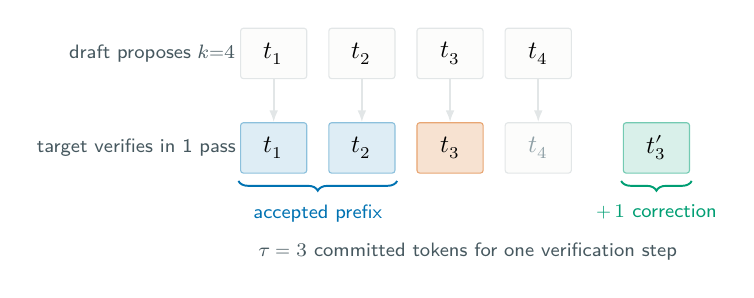
\begin{tikzpicture}[
  x=1.12cm,
  tok/.style={draw=rule, fill=surface, minimum width=8.4mm, minimum height=6.4mm,
              inner sep=0pt, font=\small, rounded corners=1pt},
  ok/.style  ={tok, fill=accent!13, draw=accent!45},
  no/.style  ={tok, fill=warm!18,   draw=warm!55},
  fix/.style ={tok, fill=teal!15,   draw=teal!55},
  gone/.style={tok, draw=rule, text=muted},
  lbl/.style ={font=\scriptsize\color{ink2}, anchor=east},
]
  % --- row 1: the draft's proposal ------------------------------
  \node[lbl] at (-0.32,0) {draft proposes $k{=}4$};
  \foreach \i/\t in {0/{$t_1$}, 1/{$t_2$}, 2/{$t_3$}, 3/{$t_4$}}
    \node[tok] (d\i) at (\i,0) {\t};

  % --- row 2: the verdicts from one verification pass -----------
  \node[lbl] at (-0.32,-1.2) {target verifies in 1 pass};
  \node[ok]   (v0) at (0,-1.2) {$t_1$};
  \node[ok]   (v1) at (1,-1.2) {$t_2$};
  \node[no]   (v2) at (2,-1.2) {$t_3$};
  \node[gone] (v3) at (3,-1.2) {$t_4$};
  \node[fix]  (v4) at (4.34,-1.2) {$t_3'$};

  \foreach \i in {0,1,2,3}
    \draw[-{Latex[length=1.5mm]}, draw=rule, line width=0.7pt] (d\i) -- (v\i);

  % --- what the cycle actually yields ---------------------------
  \draw[decorate, decoration={brace, amplitude=3.5pt, mirror},
        draw=accent, line width=0.7pt] (-0.40,-1.62) -- (1.40,-1.62);
  \node[font=\scriptsize\color{accent}, anchor=north] at (0.5,-1.80)
    {accepted prefix};
  \draw[decorate, decoration={brace, amplitude=3.5pt, mirror},
        draw=teal, line width=0.7pt] (3.94,-1.62) -- (4.74,-1.62);
  \node[font=\scriptsize\color{teal}, anchor=north] at (4.34,-1.80)
    {$+\,1$ correction};
  \node[font=\scriptsize\color{ink2}, anchor=north] at (2.2,-2.28)
    {$\tau = 3$ committed tokens for one verification step};
\end{tikzpicture}}

% Inline legend swatch for the token strip, set in running text.
% \tokenkey{fill}{draw}{label}
\newcommand{\tokenkey}[3]{%
  \tikz[baseline=-0.5ex]{\draw[fill=#1, draw=#2, rounded corners=0.8pt]
    (0,-0.075) rectangle (0.26,0.185);}\,{\scriptsize\color{ink2}#3}}


% --- notes switch -----------------------------------------------
\ifdefined\NOTESMODE
  \setbeameroption{show only notes}
  \setbeamertemplate{note page}[plain]
  \setbeamerfont{note page}{size=\footnotesize}
\else
  \setbeameroption{hide notes}
  % Presenter display instead:
  % \setbeameroption{show notes on second screen=right}
\fi
% ----------------------------------------------------------------

\deckfootline{Speculative decoding on consumer GPUs\ \ \textbullet\ \ ICECCME 2026}

\begin{document}

% ================================================================
%  Title
% ================================================================
\darkframe{%
  \vfill
  \begin{minipage}{\dimexpr\paperwidth-2\deckmargin\relax}
    \raggedright
    {\displaylight\fontsize{10}{10}\selectfont\color{onink}%
      \MakeUppercase{ICECCME 2026\ \ \textbullet\ \ Bali, Indonesia\ \ \textbullet\ \ 15--17 October}}\par
    \vskip14pt
    {\displaylight\fontsize{19}{25}\selectfont\color{surface}%
      Characterizing Speculative Decoding Dynamics\\
      for Large Language Models\\
      on Consumer-Class GPUs}\par
    \vskip16pt
    {\color{onink}\rule{40pt}{2pt}}\par
    \vskip14pt
    {\displaymedium\fontsize{12}{16}\selectfont\color{surface}%
      Samsu Sempena \quad\textcolor{muted}{\textbullet}\quad Zhuohan Cui}\par
    \vskip3pt
    {\small\color{rule}The University of Sydney}\par
  \end{minipage}
  \vfill
}
\note{%
\textbf{[0:00--0:20 | Title]}\\[2pt]
``Good morning. I'm Samsu Sempena from the University of Sydney, and this is
joint work with Zhuohan Cui. Our paper characterizes what speculative decoding
actually does on consumer-class GPUs --- the kind of hardware a practitioner
has under their desk, not in a data centre.''\\[4pt]
\emph{Cue:} give the one-line thesis up front so the audience has a hook ---
``the short version is that the \emph{policy ranking} travels between GPUs,
but the \emph{speedup} does not.''\\[4pt]
\emph{Housekeeping:} confirm the clicker works, and check whether the chair
wants questions during or after.
}

\deckdivider{The problem}{Why consumer-GPU speculative decoding needs its own measurement}

% ================================================================
\begin{frame}{Decoding is sequential, and that is the bottleneck}
  \begin{columns}[T,onlytextwidth]
    \begin{column}{0.55\textwidth}
      \begin{itemize}\itemsep6pt
        \item Autoregressive decoding needs \alert{one full forward pass of
              the target model per token}.
        \item Single-stream interactive latency is bound by \emph{memory
              traffic}, not arithmetic.
        \item Speculative decoding is the standard fix --- and is reported as
              a large, nearly free win.
      \end{itemize}
      \vskip10pt
      \begin{takeaway}
        Almost every published gain is measured on \textbf{data-centre}
        hardware. On a single RTX-class GPU, what actually happens?
      \end{takeaway}
    \end{column}
    \begin{column}{0.42\textwidth}
      {\footnotesize\color{ink2}\textsc{Open deployment questions}}\par
      \vskip5pt
      {\small
      \begin{tabular}{@{}l@{\hskip 10pt}l@{}}
        \toprule
        Which draft size?      & 0.5B? 1.5B? \\
        Which proposal length? & $k{=}4$? 8? 16? \\
        Greedy or sampling?    & speed vs.\ quality \\
        Does it transfer?      & desktop $\to$ laptop \\
        \bottomrule
      \end{tabular}}
    \end{column}
  \end{columns}
\end{frame}
\note{%
\textbf{[0:20--1:05 | Motivation]}\\[2pt]
Frame the bottleneck physically: every token costs a complete pass over the
target model's weights, so on a single stream you move gigabytes of weights per
token while the GPU's compute units sit mostly idle. That is why batch-1
interactive decoding is memory-bandwidth bound.\\[4pt]
Then pivot: ``speculative decoding is the well-known answer, and the literature
reports two- to five-times speedups. But look at where those numbers come from
--- A100s, H100s, B200s. The practitioner running a 3B or 4B model on one RTX
card has no reliable guidance.''\\[4pt]
Point at the four questions on the right --- these are exactly the knobs someone
has to set on day one --- and say we will answer all four with measurements.\\[4pt]
\emph{Do not} over-explain memory bandwidth; one sentence is enough.
}

% ================================================================
\begin{frame}{One speculative cycle}
  \centering
  \vskip-2pt
  \tokenstrip

  \vskip9pt
  \tokenkey{accent!13}{accent!45}{accepted}\quad
  \tokenkey{warm!18}{warm!55}{first mismatch}\quad
  \tokenkey{surface}{rule}{discarded}\quad
  \tokenkey{teal!15}{teal!55}{target correction}

  \vskip10pt
  \begin{columns}[T,onlytextwidth]
    \begin{column}{0.42\textwidth}
      \centering
      $\displaystyle L \;=\; \frac{T_{\text{draft}} + T_{\text{verify}}}{\tau}$
      \vskip4pt
      {\small $T_{\text{draft}} = k \cdot t_{\text{draft step}}$}
    \end{column}
    \begin{column}{0.54\textwidth}
      {\small
      Numerator grows \alert{linearly} in $k$; $\tau$ saturates as acceptance
      falls. \textbf{So some $k$ must lose.} Modified rejection sampling keeps
      the output distribution identical to the target's.}
    \end{column}
  \end{columns}
\end{frame}
\note{%
\textbf{[1:05--2:00 | Method recap]}\\[2pt]
Keep this brisk --- most of the room knows the algorithm. Walk the strip once:
the draft proposes four tokens; the target checks all four in a single pass;
here it agrees on the first two, disagrees on the third, so everything from the
mismatch onward is thrown away and the target supplies one corrected token. Net
yield: three committed tokens for one verification step.\\[4pt]
Then land on the equation, because it is the analytical spine of every result
that follows: ``the cost in the numerator grows linearly with $k$ --- you run
the draft model $k$ times. The payoff is $\tau$, and $\tau$ saturates, because
once acceptance drops off the extra proposals are wasted work. The theory
already tells you there is a crossover. Our contribution is showing
\emph{where} it sits on real consumer hardware --- and it sits much lower than
people assume.''\\[4pt]
Mention the correctness guarantee once. It pre-empts a question, and it makes
the quality result later more interesting.
}

% ================================================================
\begin{frame}{What is missing, and what we ask}
  \begin{columns}[T,onlytextwidth]
    \begin{column}{0.42\textwidth}
      {\footnotesize\color{ink2}\textsc{Three gaps}}\par
      \vskip6pt
      \begin{itemize}\itemsep5pt
        \item No cross-model \emph{and} cross-hardware validation at the
              consumer tier.
        \item Speedups reported as bare means --- no dispersion.
        \item Rarely a statistical test against a matched baseline.
      \end{itemize}
      \vskip8pt
      {\small\color{ink2}A \emph{characterization} paper, not a new decoding
      algorithm.}
    \end{column}
    \begin{column}{0.55\textwidth}
      {\footnotesize\color{ink2}\textsc{Research questions}}\par
      \vskip6pt
      {\small
      \begin{tabular}{@{}p{0.09\linewidth}@{}>{\raggedright\arraybackslash}p{0.89\linewidth}@{}}
        \textcolor{accent}{\textbf{RQ1}} & How much end-to-end speedup on consumer RTX hardware?\\[4pt]
        \textcolor{accent}{\textbf{RQ2}} & How do $k$ and acceptance \emph{jointly} set net latency?\\[4pt]
        \textcolor{accent}{\textbf{RQ3}} & How sensitive is the trade-off to deterministic vs.\ stochastic decoding?\\[4pt]
        \textcolor{accent}{\textbf{RQ4}} & Do rankings and gains transfer RTX4090 $\to$ RTX5090-laptop?\\
      \end{tabular}}
    \end{column}
  \end{columns}
\end{frame}
\note{%
\textbf{[2:00--2:40 | Gap and RQs]}\\[2pt]
Be explicit about the contribution type: ``we are not proposing a faster
drafter. We are asking whether the existing, unmodified draft--verify loop
delivers on the hardware most people actually own, and answering it with the
statistical care that a deployment decision deserves.''\\[4pt]
Read RQ1 and RQ4 aloud; gesture at RQ2 and RQ3. RQ4 is the one they will
remember, so give it a beat: ``and the fourth question is the one that
surprised us.''\\[4pt]
\emph{If running long:} skip the three gaps entirely, go straight to the RQs.
Saves about 20 seconds.
}

% ================================================================
\begin{frame}{Experimental protocol}
  \begin{columns}[T,onlytextwidth]
    \begin{column}{0.47\textwidth}
      {\footnotesize\color{ink2}\textsc{Models}\ \ (same-family pairings)}\par
      \vskip4pt
      {\small
      \begin{tabular}{@{}ll@{}}
        Qwen2.5-3B-Instruct & $\leftarrow$ 0.5B draft\\
        Qwen3-4B-Instruct   & $\leftarrow$ 0.6B draft\\
      \end{tabular}}\par
      \vskip3pt
      {\footnotesize\color{ink2}FP16, matched tokenizers, KV cache both sides.}
      \vskip11pt
      {\footnotesize\color{ink2}\textsc{Hardware}}\par
      \vskip4pt
      {\small
      \begin{tabular}{@{}l@{\hskip 8pt}N@{\hskip 8pt}N@{}}
        \toprule
                          & \textbf{RTX4090} & \textbf{RTX5090-L}\\
        \midrule
        Bandwidth (GB/s)  & 1008 & 896\\
        CUDA cores        & 16384 & 10496\\
        Power (W)         & 450 & $\leq$150\\
        \bottomrule
      \end{tabular}}
    \end{column}
    \begin{column}{0.50\textwidth}
      \begin{takeaway}
        \textbf{Fixed-policy grid.} $k \in \{4,8,16\}$ $\times$ \{det., stoch.\}
        = 6 configurations \emph{per family per device}, each against a
        \alert{regime-matched} autoregressive baseline.
      \end{takeaway}
      \vskip9pt
      {\footnotesize\color{ink2}\textsc{Controls}}\par
      \vskip4pt
      {\footnotesize\raggedright
      Deterministic $T{=}0$, top-$p{=}1$; stochastic $T{=}0.7$, top-$p{=}0.9$.\\
      1000 samples, frozen manifests: GSM8K 300, MMLU 500, CNN/DM 200.\\
      Seed 42 primary; repeat seeds 123/999 at $k{=}4$.\par}
    \end{column}
  \end{columns}
\end{frame}
\note{%
\textbf{[2:40--3:40 | Protocol]}\\[2pt]
The message here is \emph{pairing}. Every speculative run is compared against a
baseline that used the same prompts, the same sample IDs, the same length
limits and the same sampling regime --- so speedup is computed per sample, not
as a ratio of two independent averages. That is what makes the paired
$t$-tests later legitimate.\\[4pt]
Note the deliberate choice of same-family pairings: matching tokenizers means no
vocabulary-alignment overhead contaminating the measurement. Cross-family
pairing is a different study.\\[4pt]
On hardware, flag the counter-intuitive line: the laptop 5090 is the
\emph{newer} architecture --- Blackwell versus Ada --- but it has lower memory
bandwidth and roughly a third of the power budget. Plant that seed now; it pays
off at RQ4.\\[4pt]
Be honest about the seed budget: full grid at seed 42, repeats only at $k{=}4$.
Somebody will ask.
}

\deckdivider{What we measured}{Speedup, acceptance, token timing, and what transfers}

% ================================================================
\begin{frame}{RQ1 --- on the RTX4090, it works}
  \vskip-4pt
  \begin{columns}[T,onlytextwidth]
    \begin{column}{0.30\textwidth}\stattile{3.07}{$\times$}{Qwen2.5 peak, deterministic $k{=}4$}\end{column}
    \begin{column}{0.30\textwidth}\stattile[warm]{2.85}{$\times$}{Qwen3 peak, deterministic $k{=}4$}\end{column}
    \begin{column}{0.30\textwidth}\stattile[teal]{11}{\,/\,12}{Configurations above baseline}\end{column}
  \end{columns}
  \vskip12pt
  \centering
  {\small
  \begin{tabular}{@{}l@{\hskip 12pt}NN@{\hskip 14pt}NN@{\hskip 14pt}NN@{}}
    \toprule
    & \multicolumn{2}{c}{\textbf{$k=4$}} & \multicolumn{2}{c}{\textbf{$k=8$}}
    & \multicolumn{2}{c}{\textbf{$k=16$}}\\
    \cmidrule(r{10pt}){2-3}\cmidrule(r{10pt}){4-5}\cmidrule{6-7}
    \textbf{Speedup $S$} & det & stoch & det & stoch & det & stoch\\
    \midrule
    Qwen2.5 (3B $\leftarrow$ 0.5B) & \textcolor{accent}{\textbf{3.0674}} & 2.9394 & 2.4542 & 2.4063 & 1.8050 & 1.8185\\
    Qwen3 \ (4B $\leftarrow$ 0.6B) & \textcolor{accent}{\textbf{2.8548}} & 2.4798 & 1.9648 & 1.6869 & 1.1091 & \textcolor{warm}{\textbf{0.9719}}\\
    \bottomrule
  \end{tabular}}
  \vskip8pt
  {\small\color{ink2}Both families peak at the \emph{smallest} $k$ we tested.
  Qwen3 stochastic $k{=}16$ is the single loss.}
\end{frame}
\note{%
\textbf{[3:40--4:55 | RQ1 headline]}\\[2pt]
This is the good-news slide --- deliver it confidently, then immediately
complicate it.\\[4pt]
Lead with the tiles: ``just over three times on Qwen2.5, just under three on
Qwen3, both at deterministic $k{=}4$. Eleven of our twelve RTX4090
configurations beat their baseline.''\\[4pt]
Then the hook into RQ2: ``but notice which column the best numbers are in. It
is the \emph{smallest} $k$ we tested. Every step toward a longer proposal costs
us speed. And in the bottom-right cell --- Qwen3, stochastic, $k{=}16$ ---
speculative decoding is actually \emph{slower} than just running the target
model normally.''\\[4pt]
\emph{Pointer discipline:} touch three cells only --- the two peaks and the
0.9719. Do not read the table out.
}

% ================================================================
\begin{frame}{RQ2 --- bigger blocks, slower generation}
  \begin{columns}[T,onlytextwidth]
    \begin{column}{0.53\textwidth}
      \vskip2pt
      \chartFamilies{3.3cm}
      \vskip2pt
      {\centering
      \huekey{accent} {\scriptsize\color{ink2}Qwen2.5}\quad
      \huekey{warm} {\scriptsize\color{ink2}Qwen3}\quad
      \stylekey{solid} {\scriptsize\color{ink2}det.}\quad
      \stylekey{dashed} {\scriptsize\color{ink2}stoch.}\par}
    \end{column}
    \begin{column}{0.44\textwidth}
      {\footnotesize\color{ink2}\textsc{Mean speedup, $k{=}4 \to k{=}16$}}\par
      \vskip4pt
      {\small\begin{tabular}{@{}l@{\hskip 8pt}N@{\ }l@{\ }N@{}}
        Qwen2.5 & 2.9164 & $\to$ & 1.8118\\
        Qwen3   & 2.6673 & $\to$ & 1.0405\\
      \end{tabular}}
      \vskip10pt
      {\footnotesize\color{ink2}\textsc{Token timing degrades too}\ \
      \tiny(Qwen3, RTX4090, det.)}\par
      \vskip4pt
      {\small\begin{tabular}{@{}l@{\hskip 8pt}N@{\ }l@{\ }N@{\ }l@{}}
        TTFT & 132.6 & $\to$ & 349.6 & ms\\
        TPOT & 41.2  & $\to$ & 94.2  & ms/tok\\
      \end{tabular}}
      \vskip10pt
      \begin{takeawaywarm}
        $B_{\text{eff}}$ \emph{rises} ($1.33 \to 1.96$) while latency
        \emph{worsens}. The overhead inflection arrives \alert{before $k{=}8$}.
      \end{takeawaywarm}
    \end{column}
  \end{columns}
\end{frame}
\note{%
\textbf{[4:55--5:55 | RQ2 the inflection]}\\[2pt]
The analytically interesting result --- slow down here.\\[4pt]
``Our hypothesis going in --- H2 --- was the textbook one: $k{=}8$ should beat
$k{=}4$, and $k{=}16$ might start to lose. That is wrong on this hardware. All
four curves fall monotonically from the smallest $k$ we tested. The inflection
has already happened before $k{=}8$.''\\[4pt]
Explain \emph{why} with the equation from earlier: the effective block size does
go up --- you really do commit more tokens per verify step --- but sub-linearly,
while drafting cost goes up linearly. Acceptance is only 34\% at $k{=}4$ and
collapses to 13\% at $k{=}16$, so most of those extra draft steps are pure
waste.\\[4pt]
The token-timing numbers are the practitioner's punchline: at $k{=}16$ you have
nearly tripled time-to-first-token. For an interactive application that is the
worst possible place to spend latency --- the user sees it directly.\\[4pt]
\emph{Implication to state:} on this class of hardware, tune $k$ downward ---
and $k{=}4$ may not even be the floor.
}

% ================================================================
\begin{frame}{RQ3 --- deterministic decoding is the safer default}
  \begin{columns}[T,onlytextwidth]
    \begin{column}{0.50\textwidth}
      {\small
      \begin{tabular}{@{}l@{\hskip 10pt}NNN@{}}
        \toprule
        \textbf{Qwen3, RTX4090} & $k{=}4$ & $k{=}8$ & $k{=}16$\\
        \midrule
        Deterministic $S$ & 2.8548 & 1.9648 & 1.1091\\
        Stochastic $S$    & 2.4798 & 1.6869 & 0.9719\\
        \midrule
        Advantage & \textcolor{accent}{\textbf{+0.3750}} & +0.2779 & +0.1372\\
        \bottomrule
      \end{tabular}}
      \vskip12pt
      \begin{itemize}\itemsep5pt
        \small
        \item Greedy drafting agrees with greedy verification more often
              $\Rightarrow$ higher $\alpha$ (0.336 vs.\ 0.267 at $k{=}4$).
        \item The advantage \emph{shrinks} with $k$: once acceptance is low,
              the regime hardly matters.
      \end{itemize}
    \end{column}
    \begin{column}{0.46\textwidth}
      \begin{takeawaywarm}
        \textbf{Not universal.} Qwen2.5 follows the same ordering at $k{=}4$
        and $k{=}8$, then reverses slightly at $k{=}16$ --- 1.8050
        deterministic vs.\ 1.8185 stochastic.
      \end{takeawaywarm}
      \vskip10pt
      \begin{takeaway}
        If you need sampling, expect to pay about \textbf{13\% of your
        speedup} for it at low $k$.
      \end{takeaway}
    \end{column}
  \end{columns}
\end{frame}
\note{%
\textbf{[5:55--6:30 | RQ3 regime]}\\[2pt]
Short slide --- the least surprising result, so move through it.\\[4pt]
The mechanism is worth saying out loud: ``when both draft and target decode
greedily, the draft's proposal is compared against a deterministic target
continuation, so agreement is high. Turn sampling on for both and you introduce
two independent sources of randomness; acceptance drops from about 34\% to
27\%, and you lose roughly 13\% of your speedup.''\\[4pt]
State the caveat rather than hiding it: at $k{=}16$ Qwen2.5 actually reverses,
marginally. Small effect, but we report it --- the preference is a strong
tendency, not a law.\\[4pt]
\emph{If running long:} first slide to cut. Say ``deterministic wins at matched
$k$, by a margin that shrinks as $k$ grows'' and click through.
}

% ================================================================
\begin{frame}{RQ4 --- same policy, different GPU, and it all inverts}
  \begin{columns}[T,onlytextwidth]
    \begin{column}{0.53\textwidth}
      \vskip2pt
      \chartHardware{3.3cm}
      \vskip2pt
      {\centering
      \huekey{accent} {\scriptsize\color{ink2}RTX4090}\quad
      \huekey{teal} {\scriptsize\color{ink2}RTX5090-laptop}\quad
      \stylekey{solid} {\scriptsize\color{ink2}det.}\quad
      \stylekey{dashed} {\scriptsize\color{ink2}stoch.}\par}
    \end{column}
    \begin{column}{0.44\textwidth}
      \vskip6pt
      \stattile[warm]{0.67}{$\times$}{Best RTX5090-laptop configuration
      (deterministic $k{=}4$) --- all six span $0.22$--$0.67\times$}
      \vskip12pt
      \begin{takeawaywarm}
        Every configuration is \alert{slower than baseline} --- yet acceptance
        equals or beats the RTX4090 at every $k$ (0.335 vs.\ 0.336 at $k{=}4$;
        0.180 vs.\ 0.129 at $k{=}16$).\\[4pt]
        The loss is in per-step execution cost, not in the algorithm.
      \end{takeawaywarm}
    \end{column}
  \end{columns}
\end{frame}
\note{%
\textbf{[6:30--7:50 | RQ4 portability --- the core result]}\\[2pt]
This is the slide the talk exists for. Pause before starting it.\\[4pt]
``We took the identical code, the identical models, the identical frozen
manifests, and moved to an RTX5090 laptop --- a \emph{newer} architecture.
Every single configuration is now slower than simply running the target model
autoregressively. The best case, deterministic $k{=}4$, gives 0.67 --- we have
made inference about one and a half times slower.''\\[4pt]
Then the diagnostic point, which is what makes this a finding rather than an
anecdote: ``acceptance is not the problem. At $k{=}4$ it is identical --- 0.336
against 0.335. At $k{=}8$ and $k{=}16$ the laptop actually accepts \emph{more}
--- 0.25 against 0.24, and 0.18 against 0.13. So the speculative algorithm is
doing at least as well there as on the desktop, and it is still slower
everywhere. What changed is the runtime economics: the draft model's per-step
cost relative to the target's verification cost is unfavourable on this stack,
and speculative decoding needs that ratio to be small.''\\[4pt]
Land the deployment rule: ``speedup is a property of the complete
model--hardware--runtime stack. Not of the algorithm, and certainly not of the
GPU generation --- the newer card lost.''\\[4pt]
Then the constructive half: the \emph{ranking} did transfer. Low $k$ beats high
$k$, deterministic beats stochastic, on both devices. Policy exploration on one
machine is transferable; absolute claims are not.
}
\note{%
\textbf{[RQ4, continued --- questions to expect]}\\[2pt]
\emph{``Did you isolate the cause?''} No, and say so. Our candidate explanation
is host-side orchestration and graph-capture behaviour --- see the CUDA-graph
note in the paper --- but we did not measure it, so we report it as context, not
as a cause. Say this before someone asks.\\[4pt]
\emph{``Is the laptop card simply weaker?''} Partly --- lower bandwidth, roughly
a third of the power budget. But $S$ is a \emph{ratio} against that same
device's own autoregressive baseline, so a uniformly slower card should not by
itself push the ratio below one. The backup hardware slide has the numbers.\\[4pt]
\emph{``Would a better runtime fix it?''} Very likely, and that is precisely the
point: the fix lives in the stack, so the stack is what you have to measure.
}

% ================================================================
\begin{frame}{Is the effect real? Statistics and stability}
  \begin{columns}[T,onlytextwidth]
    \begin{column}{0.52\textwidth}
      {\footnotesize\color{ink2}\textsc{Paired one-sided $t$-tests}, $H_0{:}\ S \le 1$\\
       paired by sample, Holm--Bonferroni across 6 configs\\
       (Qwen3, RTX4090, $n{=}1000$)}\par
      \vskip5pt
      {\small
      \begin{tabular}{@{}l@{\hskip 10pt}l@{\hskip 10pt}l@{}}
        \toprule
        Config & $d_S$ & $p_S$\\
        \midrule
        det $k{=}4,8,16$ & \vals{1.18 / 1.10 / 0.29} & all $<10^{-18}$\\
        stoch $k{=}4,8$  & \vals{1.24 / 1.13}        & both $<10^{-179}$\\
        stoch $k{=}16$   & \textcolor{warm}{\vals{$-0.08$}} & \textcolor{warm}{\vals{0.996}}\\
        \bottomrule
      \end{tabular}}
      \vskip8pt
      \begin{takeawaywarm}
        \textbf{Dispersion is large.} Per-sample $S$ (det.) goes from
        \vals{$2.7561\pm0.5950$} at $k{=}4$ to \vals{$1.3549\pm0.6533$} at
        $k{=}16$ --- at $k{=}16$ the standard deviation is half the mean.
      \end{takeawaywarm}
    \end{column}
    \begin{column}{0.45\textwidth}
      \vskip6pt
      \chartStability{3.1cm}
      \vskip3pt
      {\centering
      \huekey{accent} {\scriptsize\color{ink2}deterministic}\quad
      \huekey{warm} {\scriptsize\color{ink2}stochastic}\par}
      \vskip6pt
      {\footnotesize\color{ink2}Repeat seeds at $k{=}4$ only: deterministic
      within 1.5\%, stochastic 0.4--5.0\%. Regime ordering preserved
      everywhere.}
    \end{column}
  \end{columns}
\end{frame}
\note{%
\textbf{[7:50--8:40 | Evidence quality]}\\[2pt]
Purpose: pre-empt the methodological objections, and show we are not
over-claiming.\\[4pt]
``Five of six RTX4090 configurations are significant after Holm--Bonferroni
correction, with large effect sizes. The sixth --- stochastic $k{=}16$ --- is
not significant, and its effect size is slightly negative, exactly consistent
with its sub-baseline mean. We report it as a null, not as noise.''\\[4pt]
The dispersion point matters more than the $p$-values: at $k{=}16$ the standard
deviation across prompts is roughly half the mean. A single reported average
speedup hides an enormous spread --- your slowest prompts may see no benefit at
all. This is one of the things the literature routinely omits.\\[4pt]
On the chart: repeat seeds at $k{=}4$. Deterministic runs move by at most 1.5\%
between seeds; stochastic by up to 5\%.\\[4pt]
\emph{Say the limitation before a reviewer does:} we only have repeat seeds at
$k{=}4$. We do not claim seed stability at $k{=}8$ or $k{=}16$.
}

% ================================================================
\begin{frame}{Speed is not free: summarization quality}
  \begin{columns}[T,onlytextwidth]
    \begin{column}{0.50\textwidth}
      \vskip4pt
      \chartQuality{3.2cm}
      \vskip3pt
      {\centering
      \huekey{warm} {\scriptsize\color{ink2}speculative $k{=}4$}\quad
      \huekey{accent} {\scriptsize\color{ink2}speculative $k{=}16$}\par}
    \end{column}
    \begin{column}{0.47\textwidth}
      {\footnotesize\color{ink2}\textsc{Deterministic, CNN/DailyMail, $n{=}200$}}\par
      \vskip5pt
      {\small
      \begin{tabular}{@{}l@{\hskip 8pt}NNN@{}}
        \toprule
                       & ROUGE-L & BLEU & BERTScore\\
        \midrule
        AR baseline    & 19.58 & 3.20 & 0.793\\
        Spec.\ $k{=}4$ & \textcolor{warm}{11.50} & \textcolor{warm}{1.39} & \textcolor{warm}{0.710}\\
        Spec.\ $k{=}16$& 14.92 & 2.04 & 0.741\\
        \bottomrule
      \end{tabular}}
      \vskip10pt
      \begin{takeawaywarm}
        The \emph{fastest} configuration is also the \emph{weakest} on
        summarization, and quality recovers as $k$ grows --- moving against
        the speed trend. A real frontier, not free acceleration.
      \end{takeawaywarm}
    \end{column}
  \end{columns}
\end{frame}
\note{%
\textbf{[8:40--9:25 | Quality trade-off]}\\[2pt]
Deliver this as an honest complication of our own headline number.\\[4pt]
``Earlier I said the peak was deterministic $k{=}4$. On summarization that is
also our \emph{worst} quality point --- ROUGE-L falls from 19.6 to 11.5, and
BLEU and BERTScore move the same way. Three independent metrics agreeing means
this is not a metric artefact.''\\[4pt]
The direction is the interesting part: quality \emph{recovers} as $k$ increases,
the opposite direction to speed. The two axes genuinely trade off across our
grid, so the operating point is a choice, not a default.\\[4pt]
\emph{Expected question --- be ready:} ``isn't speculative decoding supposed to
be distribution-preserving?'' Answer: exactly, which is why this is worth
reporting. The guarantee is about the sampling distribution under the idealized
scheme; what we measure is an end-to-end implementation on a bounded generation
budget, where accepted-prefix commitment and length limits interact. We flag it
as an observed effect in our implementation and do not claim it refutes the
theory. Do not oversell this --- it is a limitation we are surfacing.\\[4pt]
Note the chart indexes all three metrics to the baseline so they share one axis;
the absolute values are in the table beside it.
}

\deckdivider{What it means}{Bounded claims, and two rules you can deploy on}

% ================================================================
\begin{frame}{What we can and cannot claim}
  \begin{columns}[T,onlytextwidth]
    \begin{column}{0.47\textwidth}
      {\footnotesize\color{ink2}\textsc{Hypotheses}}\par
      \vskip5pt
      {\small
      \begin{tabular}{@{}p{0.08\linewidth}@{}>{\raggedright\arraybackslash}p{0.90\linewidth}@{}}
        \textbf{H1} & $S>1$ --- \textcolor{accent}{\textbf{supported}} on RTX4090 (11/12), \textcolor{warm}{\textbf{rejected}} on RTX5090-laptop.\\[4pt]
        \textbf{H2} & $k{=}8 > k{=}4$ --- \textcolor{warm}{\textbf{rejected}}; speedup falls monotonically.\\[4pt]
        \textbf{H3} & $B_{\text{eff}}$ up, latency worse --- \textcolor{accent}{\textbf{supported}}.\\[4pt]
        \textbf{H4} & Deterministic faster --- \textcolor{accent}{\textbf{mostly supported}} (one reversal).\\
      \end{tabular}}
    \end{column}
    \begin{column}{0.47\textwidth}
      {\footnotesize\color{ink2}\textsc{Threats to validity}}\par
      \vskip5pt
      \begin{itemize}\itemsep4pt\small
        \item One PyTorch/Transformers stack; no extrapolation to other
              runtimes or GPUs.
        \item Same-family Qwen pairings only.
        \item No long-context, safety, or factual-consistency evaluation.
        \item Repeat seeds cover $k{=}4$ only.
        \item CUDA-graph capture differs across run families --- reported as
              context, \emph{not} as a measured cause.
      \end{itemize}
    \end{column}
  \end{columns}
\end{frame}
\note{%
\textbf{[9:25--9:55 | Scorecard and limits]}\\[2pt]
Move quickly --- this slide is mostly for the record and for the reviewers in
the room. Do not read every bullet.\\[4pt]
Highlight two things. First, H2: ``we predicted $k{=}8$ would beat $k{=}4$ and
it does not --- the overhead inflection is earlier than the folklore
suggests.'' Second, the limitations column exists because we want the claim
bounded: one runtime stack, one model family, one benchmark suite.\\[4pt]
The CUDA-graph bullet is the intellectually honest one --- we saw a difference
in capture behaviour between run families, it is a plausible contributor to the
RTX5090 result, but we did not isolate it, so we refuse to call it the cause.\\[4pt]
\emph{Timing checkpoint:} you should be at about 9:30 here. If you are past
10:30, skip straight to the takeaways.
}

\deckstandout{Policy ranking is portable.\\[4pt] Absolute speedup is not.}
\note{%
\textbf{[9:55--10:05 | The one line]}\\[2pt]
Pause. Let it sit for two seconds. This is the sentence you want people
repeating to a colleague afterwards. Add nothing to it --- click through.
}

% ================================================================
\begin{frame}{Takeaways}
  \vskip2pt
  {\small
  \begin{enumerate}\itemsep6pt
    \item \textbf{Use a short proposal.} $k{=}4$ dominates $k{=}8$ and $k{=}16$
          on both GPUs and both families --- the inflection is earlier than
          expected.
    \item \textbf{Prefer deterministic decoding} at matched $k$; sampling costs
          about 13\% of the speedup at $k{=}4$.
    \item \textbf{Benchmark on your target stack.} RTX4090 gave $3.07\times$;
          the same code on an RTX5090 laptop was \emph{sub-baseline
          everywhere}, with acceptance equal or better.
    \item \textbf{Report dispersion and quality, not just a mean speedup.}
          Per-sample spread is large; quality moves against the speed trend.
  \end{enumerate}}
  \vskip9pt
  \begin{takeaway}
    \textbf{Future work:} the full grid across seeds, broader hardware and
    model coverage, longer contexts, factuality-sensitive metrics.
  \end{takeaway}
\end{frame}
\note{%
\textbf{[10:05--10:40 | Close]}\\[2pt]
Four sentences, one per point, then stop. Do not re-explain --- the audience has
seen all the evidence.\\[4pt]
Rule one: short proposals. Rule two: greedy if you can afford it. Rule three ---
emphasize this one with your voice: measure on the machine you will actually
deploy on, because we have a concrete counter-example where a newer GPU turned a
three-times win into a one-and-a-half-times loss. Rule four: report the spread
and the quality, because a mean speedup on its own is not a deployment
decision.\\[4pt]
Close on future work in one breath, then: ``Thank you --- I'm happy to take
questions.''
}

% ================================================================
\appendix

\deckdivider{Backup}{Full grids, acceptance portability, metrics, hardware}

\begin{frame}{Backup --- full Qwen3 RTX4090 grid}
  \centering
  {\small
  \begin{tabular}{@{}l@{\hskip 12pt}NNNNNN@{}}
    \toprule
    \textbf{Config} & $S$ & $\alpha$ & $B_{\text{eff}}$
    & $T_{\text{mean}}$ (s) & TTFT (ms) & TPOT (ms)\\
    \midrule
    $k{=}4$, det    & 2.8548 & 0.3362 & 1.33 & 4.8881  & 132.57 & 41.23\\
    $k{=}4$, stoch  & 2.4798 & 0.2672 & 1.06 & 5.6196  & 134.54 & 45.51\\
    $k{=}8$, det    & 1.9648 & 0.2378 & 1.86 & 7.1024  & 204.99 & 58.76\\
    $k{=}8$, stoch  & 1.6869 & 0.1916 & 1.50 & 8.2612  & 207.82 & 64.67\\
    $k{=}16$, det   & 1.1091 & 0.1292 & 1.96 & 12.5817 & 349.58 & 94.24\\
    $k{=}16$, stoch & 0.9719 & 0.1082 & 1.64 & 14.3390 & 354.82 & 106.03\\
    \bottomrule
  \end{tabular}}
  \vskip10pt
  {\small\color{ink2}Target Qwen3-4B-Instruct; draft Qwen3-0.6B-Instruct; $n{=}1000$.}
\end{frame}
\note{Use if asked for the full Qwen3 numbers, or for TTFT/TPOT detail.}

\begin{frame}{Backup --- full Qwen2.5 RTX4090 grid}
  \centering
  {\small
  \begin{tabular}{@{}l@{\hskip 12pt}NNNNNN@{}}
    \toprule
    \textbf{Config} & $S$ & $\alpha$ & $B_{\text{eff}}$
    & $T_{\text{mean}}$ (s) & TTFT (ms) & TPOT (ms)\\
    \midrule
    $k{=}4$, det    & 3.0674 & 0.4212 & 1.66 & 3.7210 & 102.35 & 29.06\\
    $k{=}4$, stoch  & 2.9394 & 0.4080 & 1.61 & 3.9631 & 105.26 & 30.89\\
    $k{=}8$, det    & 2.4542 & 0.3515 & 2.72 & 4.6508 & 162.76 & 36.73\\
    $k{=}8$, stoch  & 2.4063 & 0.3444 & 2.67 & 4.8411 & 165.95 & 38.04\\
    $k{=}16$, det   & 1.8050 & 0.2539 & 3.76 & 6.3234 & 277.43 & 49.34\\
    $k{=}16$, stoch & 1.8185 & 0.2516 & 3.73 & 6.4059 & 278.85 & 49.81\\
    \bottomrule
  \end{tabular}}
  \vskip10pt
  {\small\color{ink2}Target Qwen2.5-3B-Instruct; draft Qwen2.5-0.5B-Instruct; $n{=}1000$.
  Higher $\alpha$ and $B_{\text{eff}}$ than Qwen3 at every $k$.}
\end{frame}
\note{%
Qwen2.5 accepts more than Qwen3 at every $k$ --- $\alpha = 0.42$ vs.\ 0.34 at
$k{=}4$, and effective block size 3.76 vs.\ 1.96 at $k{=}16$. That is why
Qwen2.5 never falls below baseline on the RTX4090 while Qwen3 does. Likely a
smaller capability gap between the 3B target and its 0.5B draft than between
the 4B target and its 0.6B draft.
}

\begin{frame}{Backup --- full Qwen3 RTX5090-laptop grid}
  \centering
  {\small
  \begin{tabular}{@{}l@{\hskip 16pt}NNN@{}}
    \toprule
    \textbf{Config} & $S$ & $\alpha$ & $B_{\text{eff}}$\\
    \midrule
    $k{=}4$, det    & 0.6743 & 0.3353 & 1.32\\
    $k{=}4$, stoch  & 0.5924 & 0.2845 & 1.06\\
    $k{=}8$, det    & 0.4613 & 0.2538 & 1.85\\
    $k{=}8$, stoch  & 0.3995 & 0.2273 & 1.50\\
    $k{=}16$, det   & 0.2588 & 0.1803 & 1.96\\
    $k{=}16$, stoch & 0.2222 & 0.1543 & 1.64\\
    \bottomrule
  \end{tabular}}
  \vskip10pt
  {\small\color{ink2}Every configuration sits below parity, while $\alpha$ and
  $B_{\text{eff}}$ match or exceed the RTX4090 at the same $k$.}
\end{frame}
\note{%
The six RTX5090-laptop numbers behind the RQ4 chart. Note $B_{\text{eff}}$ is
identical to the RTX4090 at every $k$ (1.32/1.85/1.96 against 1.33/1.86/1.96):
the speculative loop is committing the same number of tokens per verification
step on both devices, and is still slower. That is the cleanest single piece of
evidence that the loss is in execution cost.
}

\begin{frame}{Backup --- acceptance portability}
  \begin{columns}[T,onlytextwidth]
    \begin{column}{0.55\textwidth}
      \vskip4pt
      \chartAcceptance{3.4cm}
      \vskip3pt
      {\centering
      \huekey{accent} {\scriptsize\color{ink2}RTX4090}\quad
      \huekey{teal} {\scriptsize\color{ink2}RTX5090-laptop}\quad
      \stylekey{solid} {\scriptsize\color{ink2}det.}\quad
      \stylekey{dashed} {\scriptsize\color{ink2}stoch.}\par}
    \end{column}
    \begin{column}{0.42\textwidth}
      \vskip20pt
      \begin{takeaway}
        Qwen3 acceptance on the laptop is \textbf{identical at $k{=}4$}
        (0.335 vs.\ 0.336) and \textbf{higher at $k{=}8$ and $k{=}16$}
        (0.254 vs.\ 0.238; 0.180 vs.\ 0.129).\\[5pt]
        The speculative algorithm behaves at least as well there. The
        \alert{runtime economics} are what differ.
      \end{takeaway}
    \end{column}
  \end{columns}
\end{frame}
\note{%
The most useful backup slide for the RQ4 discussion. If someone challenges the
RTX5090 result --- ``did you misconfigure it?'' --- this is the answer:
acceptance is a model-level quantity, it is unchanged at $k{=}4$ and actually
\emph{better} at higher $k$, so the speculative loop is doing at least as well
as on the desktop. The loss is in per-step execution cost, not in the algorithm.
}

\begin{frame}{Backup --- success criteria and metrics}
  \begin{columns}[T,onlytextwidth]
    \begin{column}{0.47\textwidth}
      {\footnotesize\color{ink2}\textsc{Stated success criteria}}\par
      \vskip5pt
      \begin{itemize}\itemsep4pt\small
        \item Primary: mean $S \ge 1.3\times$ with Holm--Bonferroni-corrected
              $p_S < 0.05$.
        \item Primary: absolute quality drop $\le 1.0$ point on GSM8K and
              MMLU, deterministic regime.
        \item Secondary: best $(k, \text{regime})$ under quality constraints;
              dispersion; seed stability; cross-hardware ranking transfer.
      \end{itemize}
    \end{column}
    \begin{column}{0.47\textwidth}
      {\footnotesize\color{ink2}\textsc{Key metric definitions}}\par
      \vskip5pt
      \begin{itemize}\itemsep4pt\small
        \item $S$ = baseline latency / speculative latency
        \item $\alpha$ = accepted / proposed draft tokens
        \item $B_{\text{eff}}$ = accepted draft tokens / verify steps
        \item TTFT = first token time $-$ request start
        \item TPOT = (completion $-$ first token) / output tokens
        \item $d_S$ = Cohen's $d$, paired baseline vs.\ speculative latency
      \end{itemize}
    \end{column}
  \end{columns}
\end{frame}
\note{Reference slide for methodology questions.}

\begin{frame}{Backup --- hardware profiles}
  \centering
  {\small
  \begin{tabular}{@{}l@{\hskip 16pt}l@{\hskip 16pt}l@{}}
    \toprule
    \textbf{Component} & \textbf{RTX4090 desktop} & \textbf{RTX5090 laptop}\\
    \midrule
    GPU memory       & 24\,GB GDDR6X & 24\,GB GDDR7\\
    Memory bandwidth & \textcolor{accent}{\textbf{1008\,GB/s}} & 896\,GB/s\\
    CUDA cores       & \textcolor{accent}{\textbf{16384}} & 10496\\
    Architecture     & Ada Lovelace & \textcolor{teal}{\textbf{Blackwell}}\\
    Power profile    & \textcolor{accent}{\textbf{450\,W TGP class}} & up to 150\,W TGP (OEM-dependent)\\
    Software stack   & \multicolumn{2}{c}{PyTorch + Transformers, pinned per run family}\\
    \bottomrule
  \end{tabular}}
  \vskip12pt
  {\small\color{ink2}The laptop part is the \emph{newer} architecture but has
  lower bandwidth and roughly \alert{one third of the power budget}.}
\end{frame}
\note{%
The obvious question after RQ4 is ``is the 5090 laptop just a weaker card?''
Partly --- lower bandwidth, far lower sustained power. But that affects the
autoregressive baseline too, and $S$ is a \emph{ratio} against that same
device's baseline. A uniformly slower card should not by itself flip the ratio
below 1. That is why we point at the draft/target cost ratio and the runtime
path rather than at raw card performance.
}

\end{document}
